\section{CFGs for M\~aori Language}

\subsection{CFG}

\begin{small}
  \begin{verbatim}
    S -> VP NP PP

    VP -> TAM V | TAM V TAM
    PP -> PREP-ACC NPOBJ | NPOBJ
    
    NP -> DET N | DET PN | N | PN
    NPOBJ -> DET N | DET PN | N | PN
    
    TAM -> TAM-PST | TAM-PROG | TAM-OPT | TAM-HABITUAL | TAM-DIRECTIONAL
    
    TAM-PST -> "Kua"
    TAM-PROG -> "Te" | "nei"
    TAM-OPT -> "Kia"
    TAM-HABITUAL -> "E" | "ana"
    TAM-DIRECTIONAL -> "ake"
    
    V -> "tunu" | "'aere" | "orāna" | "reka"
    DET -> "a" | "te"
    PN -> "Tere" | "Rarotonga"
    PREP-ACC -> "i" | "ki"
    N -> "'are" "maki" | "taro" | "va'ine" | "'aere" | "kōtou" | "kātoatoa" | "koe" | "'ānani"
  \end{verbatim}
\end{small}

\subsection{Results on Provided Sentences}

% sentences_maori = {
%     "Tere planted the taro": "Kua tunu a Tere i te taro",
%     "The woman is going to the hospital": "Te 'aere nei te va'ine ki te 'are maki",
%     "Hi everyone!": "Kia orāna kōtou kātoatoa",
%     "Do you like oranges?": "E reka ana koe i te 'ānani",
%     "Have you been to Rarotonga?": "Kua 'aere ake koe ki Rarotonga"
% }

\begin{enumarabic}
  \item \emph{"Kua tunu a Tere i te taro"} ("Tere planted the taro")
    
    \begin{figure}[H]
      \centering
      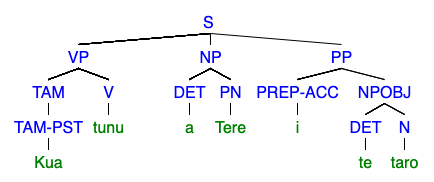
\includegraphics[width=0.7\textwidth]{figures/1.1.png}
      \caption{Parse tree for "Kua tunu a Tere i te taro"}
    \end{figure}

    \begin{figure}[H]
      \centering
      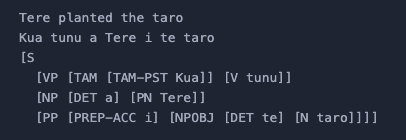
\includegraphics[width=0.7\textwidth]{figures/1.1b.png}
      \caption{Parse tree for "Kua tunu a Tere i te taro"}
    \end{figure}

  \newpage
  \item \emph{"Te 'aere nei te va'ine ki te 'are maki"} ("The woman is going to the hospital")
      
    \begin{figure}[H]
      \centering
      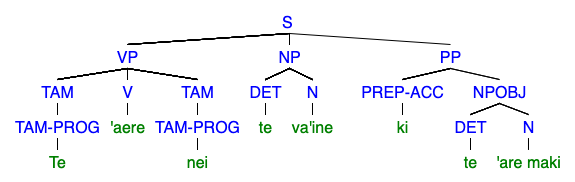
\includegraphics[width=0.7\textwidth]{figures/1.2.png}
      \caption{Parse tree for "Te 'aere nei te va'ine ki te 'are maki"}
    \end{figure}

    \begin{figure}[H]
      \centering
      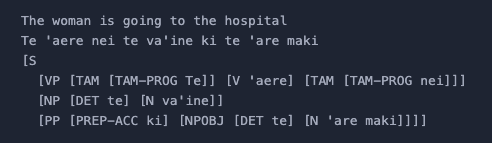
\includegraphics[width=0.7\textwidth]{figures/1.2b.png}
      \caption{Parse tree for "Te 'aere nei te va'ine ki te 'are maki"}
    \end{figure}

  \newpage
  \item \emph{"Kia orāna kōtou kātoatoa"} ("Hi everyone!")
        
    \begin{figure}[H]
      \centering
      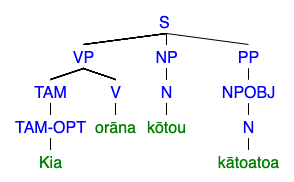
\includegraphics[width=0.7\textwidth]{figures/1.3.png}
      \caption{Parse tree for "Kia orāna kōtou kātoatoa"}
    \end{figure}

    \begin{figure}[H]
      \centering
      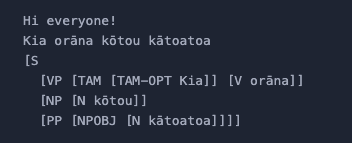
\includegraphics[width=0.7\textwidth]{figures/1.3b.png}
      \caption{Parse tree for "Kia orāna kōtou kātoatoa"}
    \end{figure}

  \newpage
  \item \emph{"E reka ana koe i te 'ānani"} ("Do you like oranges?")
            
    \begin{figure}[H]
      \centering
      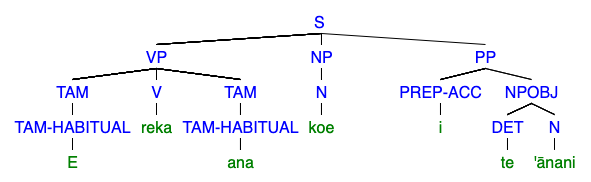
\includegraphics[width=0.7\textwidth]{figures/1.4.png}
      \caption{Parse tree for "E reka ana koe i te 'ānani"}
    \end{figure}

    \begin{figure}[H]
      \centering
      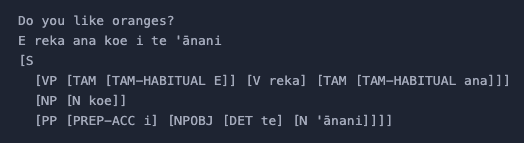
\includegraphics[width=0.7\textwidth]{figures/1.4b.png}
      \caption{Parse tree for "E reka ana koe i te 'ānani"}
    \end{figure}

  \item \emph{"Kua 'aere ake koe ki Rarotonga"} ("Have you been to Rarotonga?")

    \begin{figure}[H]
      \centering
      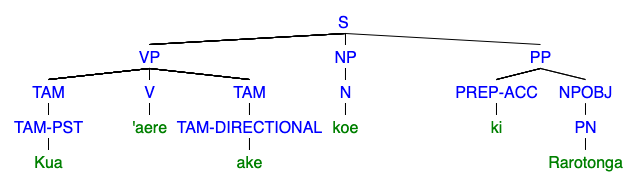
\includegraphics[width=0.7\textwidth]{figures/1.5.png}
      \caption{Parse tree for "Kua 'aere ake koe ki Rarotonga"}
    \end{figure}

    \begin{figure}[H]
      \centering
      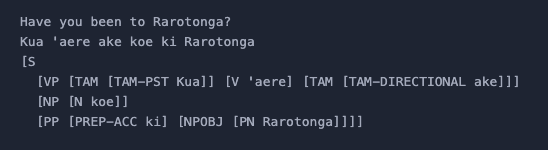
\includegraphics[width=0.7\textwidth]{figures/1.5b.png}
      \caption{Parse tree for "Kua 'aere ake koe ki Rarotonga"}
    \end{figure}
    
\end{enumarabic}
